%% Creator: Inkscape inkscape 0.92.2, www.inkscape.org
%% PDF/EPS/PS + LaTeX output extension by Johan Engelen, 2010
%% Accompanies image file 'fle4.eps' (pdf, eps, ps)
%%
%% To include the image in your LaTeX document, write
%%   \input{<filename>.pdf_tex}
%%  instead of
%%   \includegraphics{<filename>.pdf}
%% To scale the image, write
%%   \def\svgwidth{<desired width>}
%%   \input{<filename>.pdf_tex}
%%  instead of
%%   \includegraphics[width=<desired width>]{<filename>.pdf}
%%
%% Images with a different path to the parent latex file can
%% be accessed with the `import' package (which may need to be
%% installed) using
%%   \usepackage{import}
%% in the preamble, and then including the image with
%%   \import{<path to file>}{<filename>.pdf_tex}
%% Alternatively, one can specify
%%   \graphicspath{{<path to file>/}}
%% 
%% For more information, please see info/svg-inkscape on CTAN:
%%   http://tug.ctan.org/tex-archive/info/svg-inkscape
%%
\begingroup%
  \makeatletter%
  \providecommand\color[2][]{%
    \errmessage{(Inkscape) Color is used for the text in Inkscape, but the package 'color.sty' is not loaded}%
    \renewcommand\color[2][]{}%
  }%
  \providecommand\transparent[1]{%
    \errmessage{(Inkscape) Transparency is used (non-zero) for the text in Inkscape, but the package 'transparent.sty' is not loaded}%
    \renewcommand\transparent[1]{}%
  }%
  \providecommand\rotatebox[2]{#2}%
  \ifx\svgwidth\undefined%
    \setlength{\unitlength}{632.22074835bp}%
    \ifx\svgscale\undefined%
      \relax%
    \else%
      \setlength{\unitlength}{\unitlength * \real{\svgscale}}%
    \fi%
  \else%
    \setlength{\unitlength}{\svgwidth}%
  \fi%
  \global\let\svgwidth\undefined%
  \global\let\svgscale\undefined%
  \makeatother%
  \begin{picture}(1,0.45553708)%
    \put(0,0){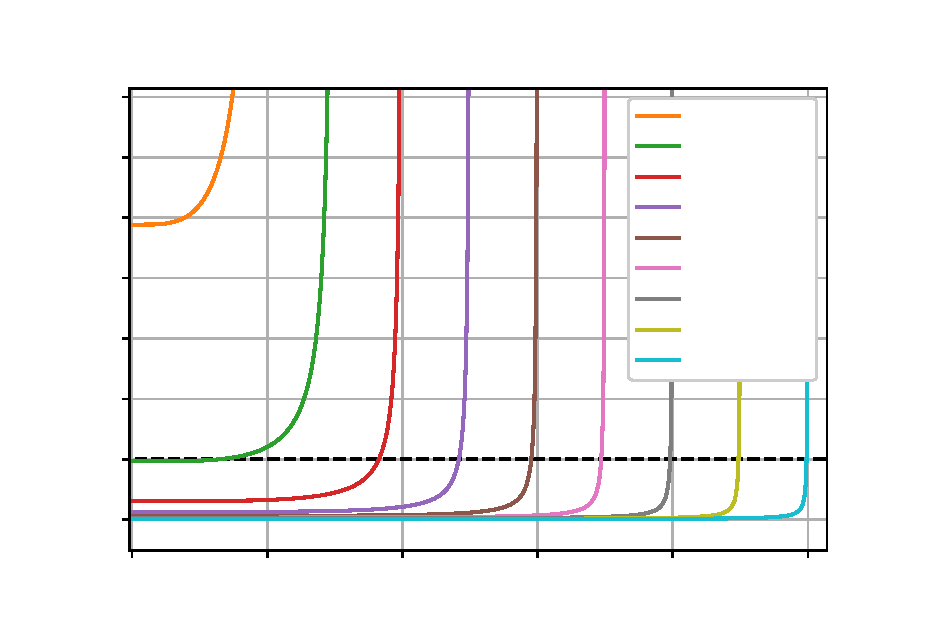
\includegraphics[width=\unitlength]{images_2ddl/fle4.eps}}%
    \put(0.12,0.02702584){\color[rgb]{0,0,0}\makebox(0,0)[lb]{\smash{0}}}%
    \put(0.26,0.02702584){\color[rgb]{0,0,0}\makebox(0,0)[lb]{\smash{10}}}%
    \put(0.41,0.02702584){\color[rgb]{0,0,0}\makebox(0,0)[lb]{\smash{20}}}%
    \put(0.56,0.02702584){\color[rgb]{0,0,0}\makebox(0,0)[lb]{\smash{30}}}%
    \put(0.71,0.02702584){\color[rgb]{0,0,0}\makebox(0,0)[lb]{\smash{40}}}%
    \put(0.86,0.02702584){\color[rgb]{0,0,0}\makebox(0,0)[lb]{\smash{50}}}%
    \put(0.06,0.1){\color[rgb]{0,0,0}\makebox(0,0)[lb]{\smash{0.0}}}%
    \put(0.06,0.165){\color[rgb]{0,0,0}\makebox(0,0)[lb]{\smash{0.1}}}%
    \put(0.06,0.23){\color[rgb]{0,0,0}\makebox(0,0)[lb]{\smash{0.2}}}%
    \put(0.06,0.3){\color[rgb]{0,0,0}\makebox(0,0)[lb]{\smash{0.3}}}%
    \put(0.06,0.365){\color[rgb]{0,0,0}\makebox(0,0)[lb]{\smash{0.4}}}%
    \put(0.06,0.435){\color[rgb]{0,0,0}\makebox(0,0)[lb]{\smash{0.5}}}%
    \put(0.06,0.5){\color[rgb]{0,0,0}\makebox(0,0)[lb]{\smash{0.6}}}%
    \put(0.06,0.565){\color[rgb]{0,0,0}\makebox(0,0)[lb]{\smash{0.7}}}%
    \put(0.03,0.3){\color[rgb]{0,0,0}\rotatebox{90}{\makebox(0,0)[lb]{\smash{$\delta / R$}}}}%
    \put(0.445,0.0){\color[rgb]{0,0,0}\makebox(0,0)[lb]{\smash{$r_1(mm)$}}}%
    \put(0.74,0.55){\color[rgb]{0,0,0}\makebox(0,0)[lb]{\smash{\footnotesize $r_2=10 mm$}}}%
    \put(0.74,0.515){\color[rgb]{0,0,0}\makebox(0,0)[lb]{\smash{\footnotesize $r_2=15 mm$}}}%
    \put(0.74,0.48){\color[rgb]{0,0,0}\makebox(0,0)[lb]{\smash{\footnotesize $r_2=20 mm$}}}%
    \put(0.74,0.445){\color[rgb]{0,0,0}\makebox(0,0)[lb]{\smash{\footnotesize $r_2=25 mm$}}}%
    \put(0.74,0.413){\color[rgb]{0,0,0}\makebox(0,0)[lb]{\smash{\footnotesize $r_2=30 mm$}}}%
    \put(0.74,0.38){\color[rgb]{0,0,0}\makebox(0,0)[lb]{\smash{\footnotesize $r_2=35 mm$}}}%
    \put(0.74,0.345){\color[rgb]{0,0,0}\makebox(0,0)[lb]{\smash{\footnotesize $r_2=40 mm$}}}%
    \put(0.74,0.31){\color[rgb]{0,0,0}\makebox(0,0)[lb]{\smash{\footnotesize $r_2=45 mm$}}}%
    \put(0.74,0.275){\color[rgb]{0,0,0}\makebox(0,0)[lb]{\smash{\footnotesize $r_2=50 mm$}}}%
  \end{picture}%
\endgroup%
